\documentclass{standalone}
% This file was created with tikzplotlib v0.9.15.

\usepackage{siunitx}
\usepackage{pgfplots}
% and optionally (as of Pgfplots 1.3):
\pgfplotsset{compat=newest}
\pgfplotsset{plot coordinates/math parser=false}
\newlength\figureheight
\newlength\figurewidth

\newcommand{\Set}[1]{\mathcal{#1}}
\newcommand{\Vector}[1]{\bm{\MakeLowercase{#1}}}
\newcommand{\Operator}[1]{\bm{\MakeUppercase{#1}}}
%%%%%%%%%%
\DeclareMathAlphabet{\mathsfbr}{OT1}{cmss}{m}{n}%for math sans serif (cmss)
\SetMathAlphabet{\mathsfbr}{bold}{OT1}{cmss}{bx}{n}%for math sans serif (cmss)
\DeclareRobustCommand{\msf}[1]{%
  \ifcat\noexpand#1\relax\msfgreek{#1}\else\mathsfbr{#1}\fi%for math sans serif (cmss)
}
\DeclareFontEncoding{LGR}{}{} % or load \usepackage{textgreek}
\DeclareSymbolFont{sfgreek}{LGR}{cmss}{m}{n}
\SetSymbolFont{sfgreek}{bold}{LGR}{cmss}{bx}{n}
\DeclareMathSymbol{\sXi}{\mathalpha}{sfgreek}{`X}
\DeclareMathSymbol{\sUpsilon}{\mathalpha}{sfgreek}{`U}

\begin{document}

% This file was created with tikzplotlib v0.9.15.
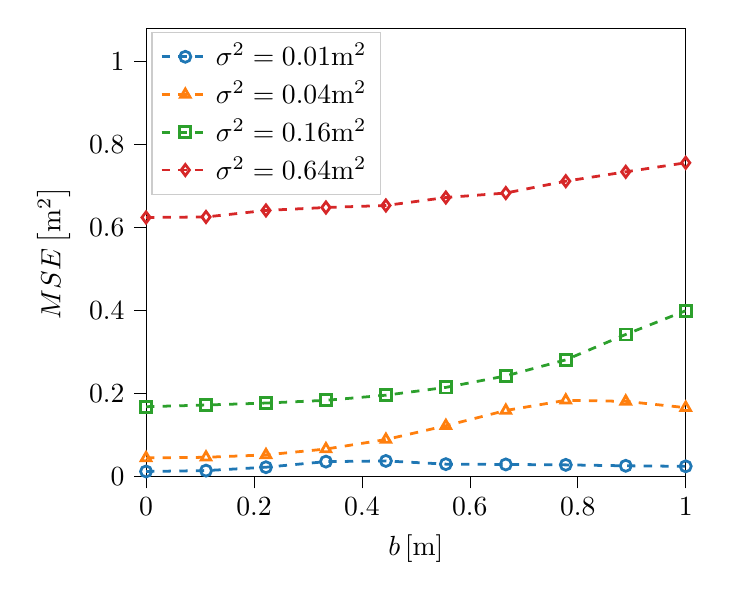
\begin{tikzpicture}

\definecolor{color0}{rgb}{0.12156862745098,0.466666666666667,0.705882352941177}
\definecolor{color1}{rgb}{1,0.498039215686275,0.0549019607843137}
\definecolor{color2}{rgb}{0.172549019607843,0.627450980392157,0.172549019607843}
\definecolor{color3}{rgb}{0.83921568627451,0.152941176470588,0.156862745098039}

\begin{axis}[
legend cell align={left},
legend style={
  fill opacity=0.8,
  draw opacity=1,
  text opacity=1,
  at={(0.01,0.81)},
  anchor=west,
  draw=white!80!black
},
tick align=outside,
tick pos=left,
x grid style={white!69.0196078431373!black},
xlabel={$b \left[ \si{m} \right]$},
xmin=0, xmax=1,
xtick style={color=black},
y grid style={white!69.0196078431373!black},
ylabel={$MSE \left[ \si{m^2} \right]$},
ymin=0, ymax=1.08,
ytick style={color=black}
]
\addplot [dashed, semithick, color0, line width=1, mark=o, mark options={solid, color0}, mark repeat=1]
table {%
0 0.01224275
0.111111111111111 0.014325
0.222222222222222 0.02245375
0.333333333333333 0.0359385
0.444444444444444 0.0375855
0.555555555555556 0.02988925
0.666666666666667 0.029118
0.777777777777778 0.02810325
0.888888888888889 0.02586275
1 0.02463375
};
\addlegendentry{$\sigma^2 = 0.01 \si{m^2}$}
\addplot [dashed, semithick, color1, line width=1, mark=triangle, mark options={solid, color1}, mark repeat=1]
table {%
0 0.0448455
0.111111111111111 0.046359
0.222222222222222 0.0521785
0.333333333333333 0.06627425
0.444444444444444 0.089074
0.555555555555556 0.122364
0.666666666666667 0.15912275
0.777777777777778 0.18369625
0.888888888888889 0.18109175
1 0.165954
};
\addlegendentry{$\sigma^2 = 0.04 \si{m^2}$}
\addplot [dashed, semithick, color2, line width=1, mark=square, mark options={solid, color2}, mark repeat=1]
table {%
0 0.16822875
0.111111111111111 0.172284
0.222222222222222 0.1770425
0.333333333333333 0.1835995
0.444444444444444 0.19598525
0.555555555555556 0.21474675
0.666666666666667 0.242403
0.777777777777778 0.281128
0.888888888888889 0.34232425
1 0.39945475
};
\addlegendentry{$\sigma^2 = 0.16 \si{m^2}$}
\addplot [dashed, semithick, color3, line width=1, mark=diamond, mark options={solid, color3}, mark repeat=1]
table {%
0 0.62410925
0.111111111111111 0.62533625
0.222222222222222 0.6410945
0.333333333333333 0.64812725
0.444444444444444 0.65300525
0.555555555555556 0.67218425
0.666666666666667 0.6829975
0.777777777777778 0.711509
0.888888888888889 0.73405025
1 0.7558055
};
\addlegendentry{$\sigma^2 = 0.64 \si{m^2}$}
\end{axis}

\end{tikzpicture}

\end{document}